% TAES paper skeleton. Journal template TBD -- swap the documentclass when the target is fixed.
\documentclass[11pt]{article}
\usepackage[margin=1in]{geometry}
\usepackage{amsmath,amssymb,booktabs,graphicx,hyperref}
\newcommand{\todo}[1]{\textbf{[TODO: #1]}}
\DeclareMathOperator{\topk}{Top\text{-}k}

\title{TAES: Timestep-Aware Expert Selection for Pretrained Diffusion Mixture-of-Experts}
\author{Mohammed Sarim}
\date{}

\begin{document}
\maketitle

\begin{abstract}
\todo{written last}
\end{abstract}

\section{Introduction}
\todo{week 7}

\section{Related Work}
\todo{week 5}

\section{Method}\label{sec:method}

\subsection{Setting}
We start from a pretrained diffusion transformer whose feed-forward layers are sparse mixtures of experts.
Each MoE layer $l\in\{1,\dots,L\}$ holds $N$ routed experts $f_{l,1},\dots,f_{l,N}$ and one always-active shared expert.
A router produces per-token logits $r_l(x)\in\mathbb{R}^N$; token $x$ is sent to the set $A_l(x)=\topk(\sigma(r_l(x)))$ of $k_0$ experts, and the layer output combines the selected expert outputs weighted by the (renormalised) gate scores.
The model is a rectified-flow model: with data latent $z_1$ and noise $z_0\sim\mathcal{N}(0,I)$, the input at time $t\in[0,1]$ is $z_t=t\,z_1+(1-t)\,z_0$, so $t=0$ is pure noise and $t=1$ is clean data.
Our aim is to select, \emph{after training and without gradients}, a subset of experts $S_{d,b,l}\subseteq\{1,\dots,N\}$ for each domain $d$, timestep band $b$ and layer $l$.
The shared expert is never selected against: with a shared expert present it replaces the residual path inside the MoE block, so removing it would sever the block's identity connection.

\paragraph{Instantiation.}
We use DSMoE-S-E48 (EMA weights): $N=48$, $k_0=5$, $L=6$ MoE layers (blocks $1,3,\dots,11$ of 12), hidden size 384, expert width 128, ImageNet $256\times256$ in a $32\times32\times4$ VAE latent space, 256 tokens per image.

\subsection{Calibration}\label{sec:calib}
For a domain $d$ (a set of ImageNet classes; here \emph{animals} and \emph{vehicles}) we take $M=500$ in-domain images, encode each once with the VAE (deterministic posterior mode, scaled by $0.18215$) and cache the latent $z_1^{(i)}$.
The unit interval is divided into $F=50$ equal fine bins. For every image and every fine bin $u$ we draw $t\sim\mathcal{U}$ within the bin and fresh noise $z_0$, form $z_t$, and run \emph{one} forward pass with the image's class label, without gradients.
Every image therefore contributes to every timestep bin ($M\cdot F=25{,}000$ forward passes per domain).
Forward hooks accumulate, per $(d,u,l,e)$, only running sums:
\begin{align*}
n &= \#\{\text{tokens routed to } e\}, \
g &= \textstyle\sum \sigma(r_{l}(x))_e \;\text{ over those tokens}, \
h &= \textstyle\sum \lVert f_{l,e}(x)\rVert_2 \;\text{ over those tokens}.
\end{align*}
Two implementation points matter. First, $g$ uses the \emph{pre-normalisation} sigmoid score: the model renormalises the selected top-$k_0$ scores to a fixed sum, which erases the router's absolute confidence, so the returned weights cannot be used. Second, $h$ is measured on the raw expert output before the gate multiplication, so the gate does not enter the score twice.
Calibration uses the conditional branch only; the unconditional branch used by classifier-free guidance at sampling time is not part of the statistics.

\subsection{Banded importance}\label{sec:score}
Partition the $F$ fine bins into $B$ contiguous bands (band $0$ the noisiest); band $b$ covers fine bins $\mathcal{U}_b$ with boundaries $\mathrm{round}(bF/B)$.
Sums are pooled over the bins of the band \emph{before} ratios are formed: $n_{b}=\sum_{u\in\mathcal{U}_b}n_u$, and likewise $g_b,h_b$.
The importance of expert $e$ is
\begin{equation}
I(e\mid d,b,l)=\underbrace{n_b}_{\text{frequency}}\cdot\underbrace{\frac{g_b}{n_b}}_{\text{mean gate}}\cdot\underbrace{\frac{h_b}{n_b}}_{\text{mean output norm}}
\;=\;\frac{g_b\,h_b}{n_b},
\end{equation}
normalised to sum to one over experts within each $(d,b,l)$ so that layers are comparable; $I=0$ if $n_b=0$.
The multiplicative form follows LLM expert-pruning scores; the timestep banding is the addition here. Because only raw sums are stored, $B$ is a free post-hoc parameter ($B=1$ recovers the global, timestep-agnostic score).

\subsection{Selection}
For a budget of $k$ experts per layer, $S_{d,b,l}$ is the set of $k$ experts with largest $I(\cdot\mid d,b,l)$, subject to $k\ge k_0$ (the router must still find $k_0$ experts).

\subsection{Deployment modes}
\paragraph{Compute mode.} At a denoising step with time $t$ in band $b$, router scores of experts outside $S_{d,b,l}$ are masked before the top-$k_0$ selection. All weights stay resident; per-step active compute is unchanged in count but restricted to the band's subset, and the rest can be offloaded.
\paragraph{Memory mode.} Take the union $U_{d,l}=\bigcup_b S_{d,b,l}$, delete all other routed experts from the checkpoint, and slice the router's output projection accordingly. The result is a physically smaller checkpoint. Its size is governed by the union, so we report the union fraction $|U_{d,l}|/N$ as a function of $k$; when bands select very different experts the union saturates towards $N$ and memory savings vanish, whereas compute mode is unaffected.
Memory reductions are reported as a fraction of routed-expert parameters; the shared expert sets a floor of $1/(N+1)$ of the MoE-layer expert parameters.

\subsection{Diagnostics}
Before any pruning we measure (i) the importance map over (expert, fine bin); (ii) the Jaccard overlap $J(S_{b},S_{b'})=|S_b\cap S_{b'}|/|S_b\cup S_{b'}|$ between bands, against the chance value for random size-$k$ subsets, $\approx (k^2/N)/(2k-k^2/N)$; and (iii) the union fraction $|\bigcup_b S_b|/N$ against $k$.
Figures~\ref{fig:heat}--\ref{fig:union} show these for the calibrated model.
\todo{quote Jaccard only after a split-half noise-floor null (Phase 4); tail experts carry little mass.}

\begin{figure}[t]\centering
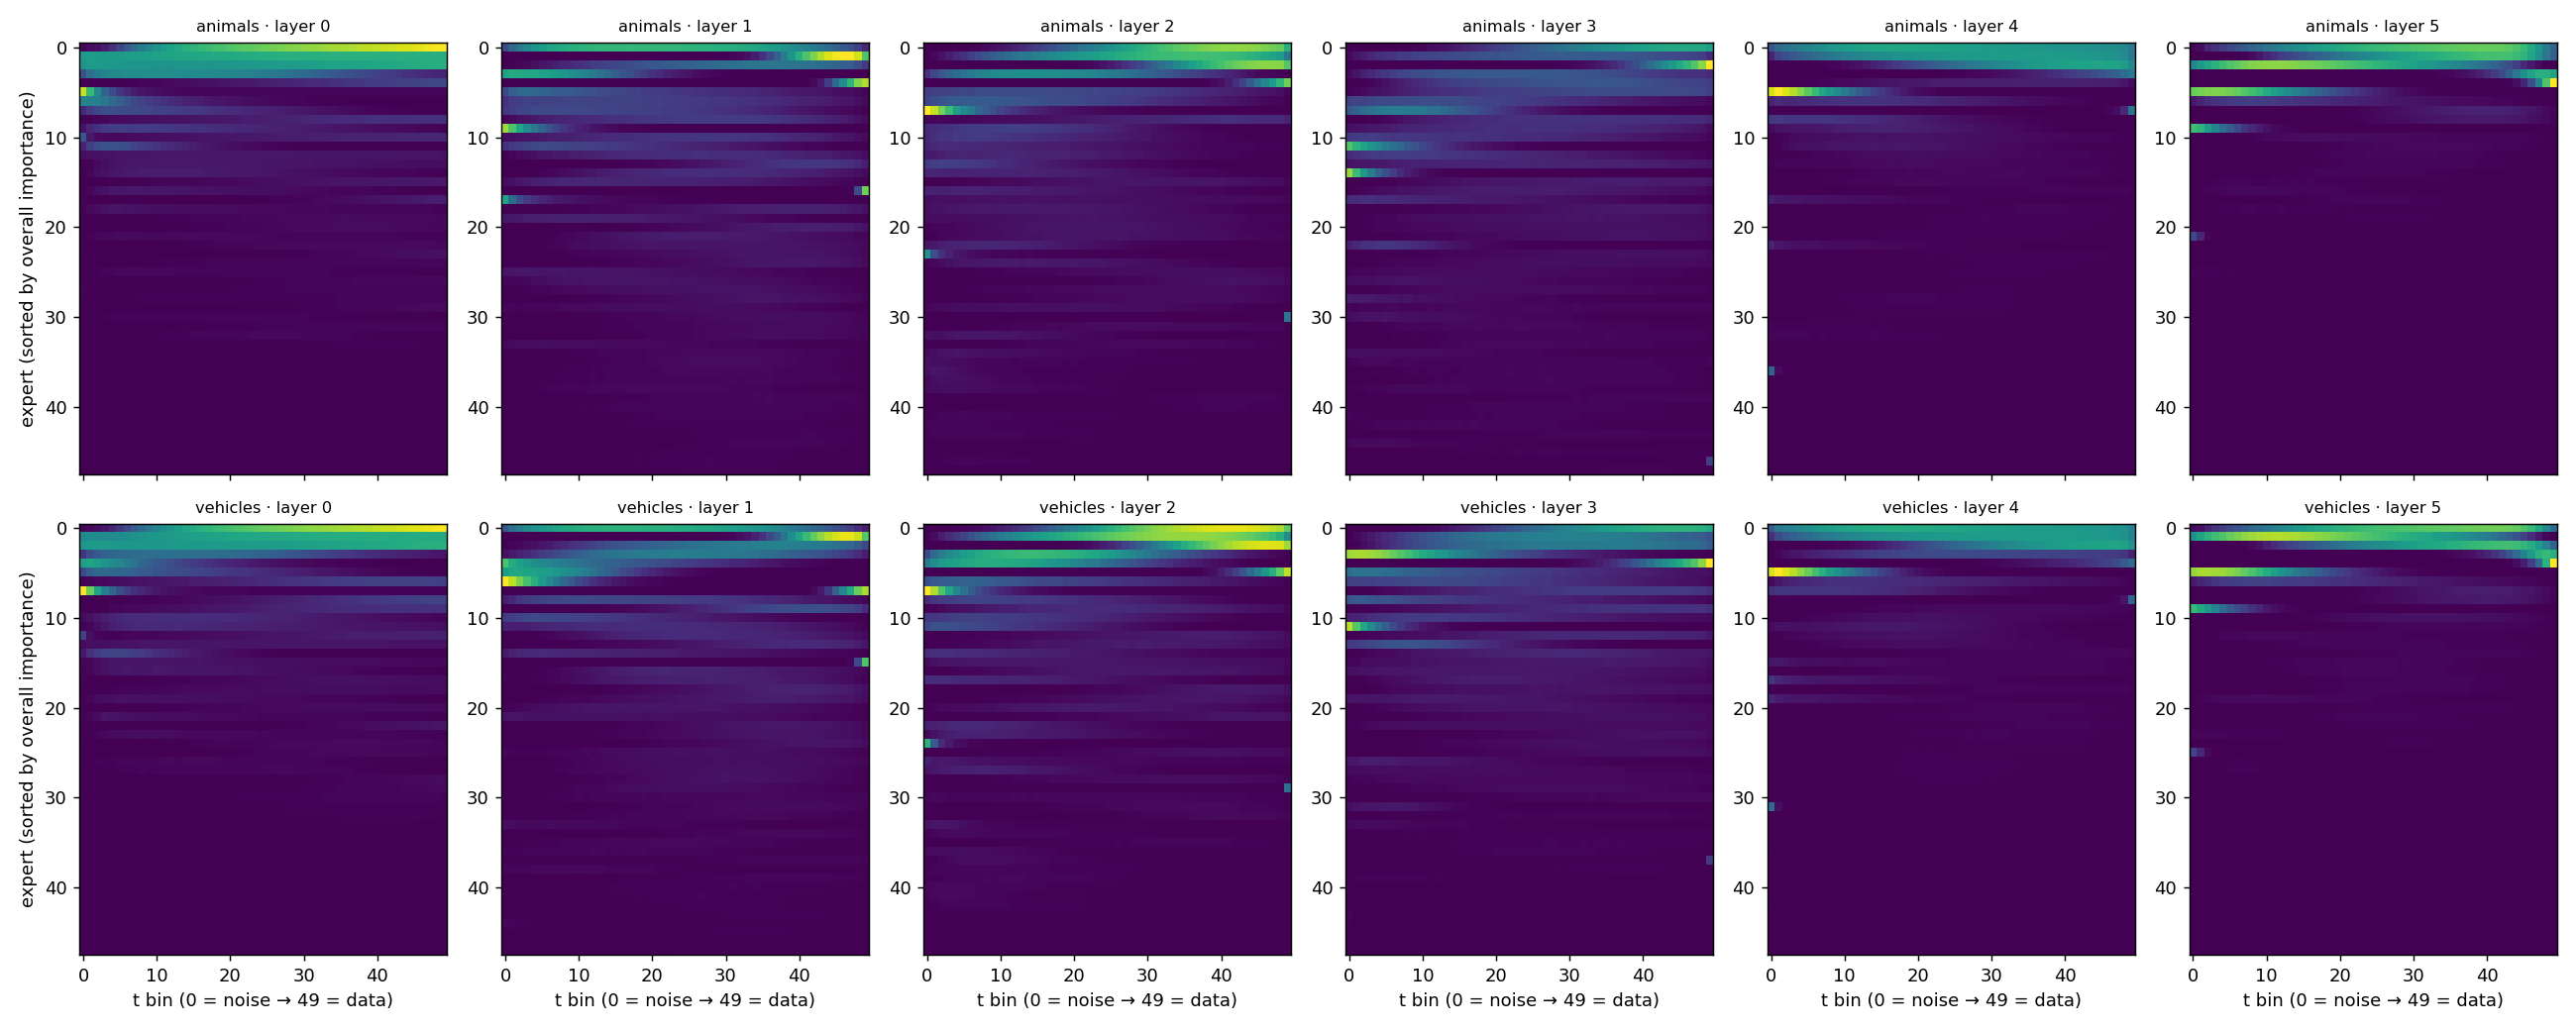
\includegraphics[width=\linewidth]{figures/diagnostic_1.png}
\caption{Expert importance over timestep bins (0 = noise, 49 = data), per layer and domain; experts sorted by global importance.}\label{fig:heat}
\end{figure}
\begin{figure}[t]\centering
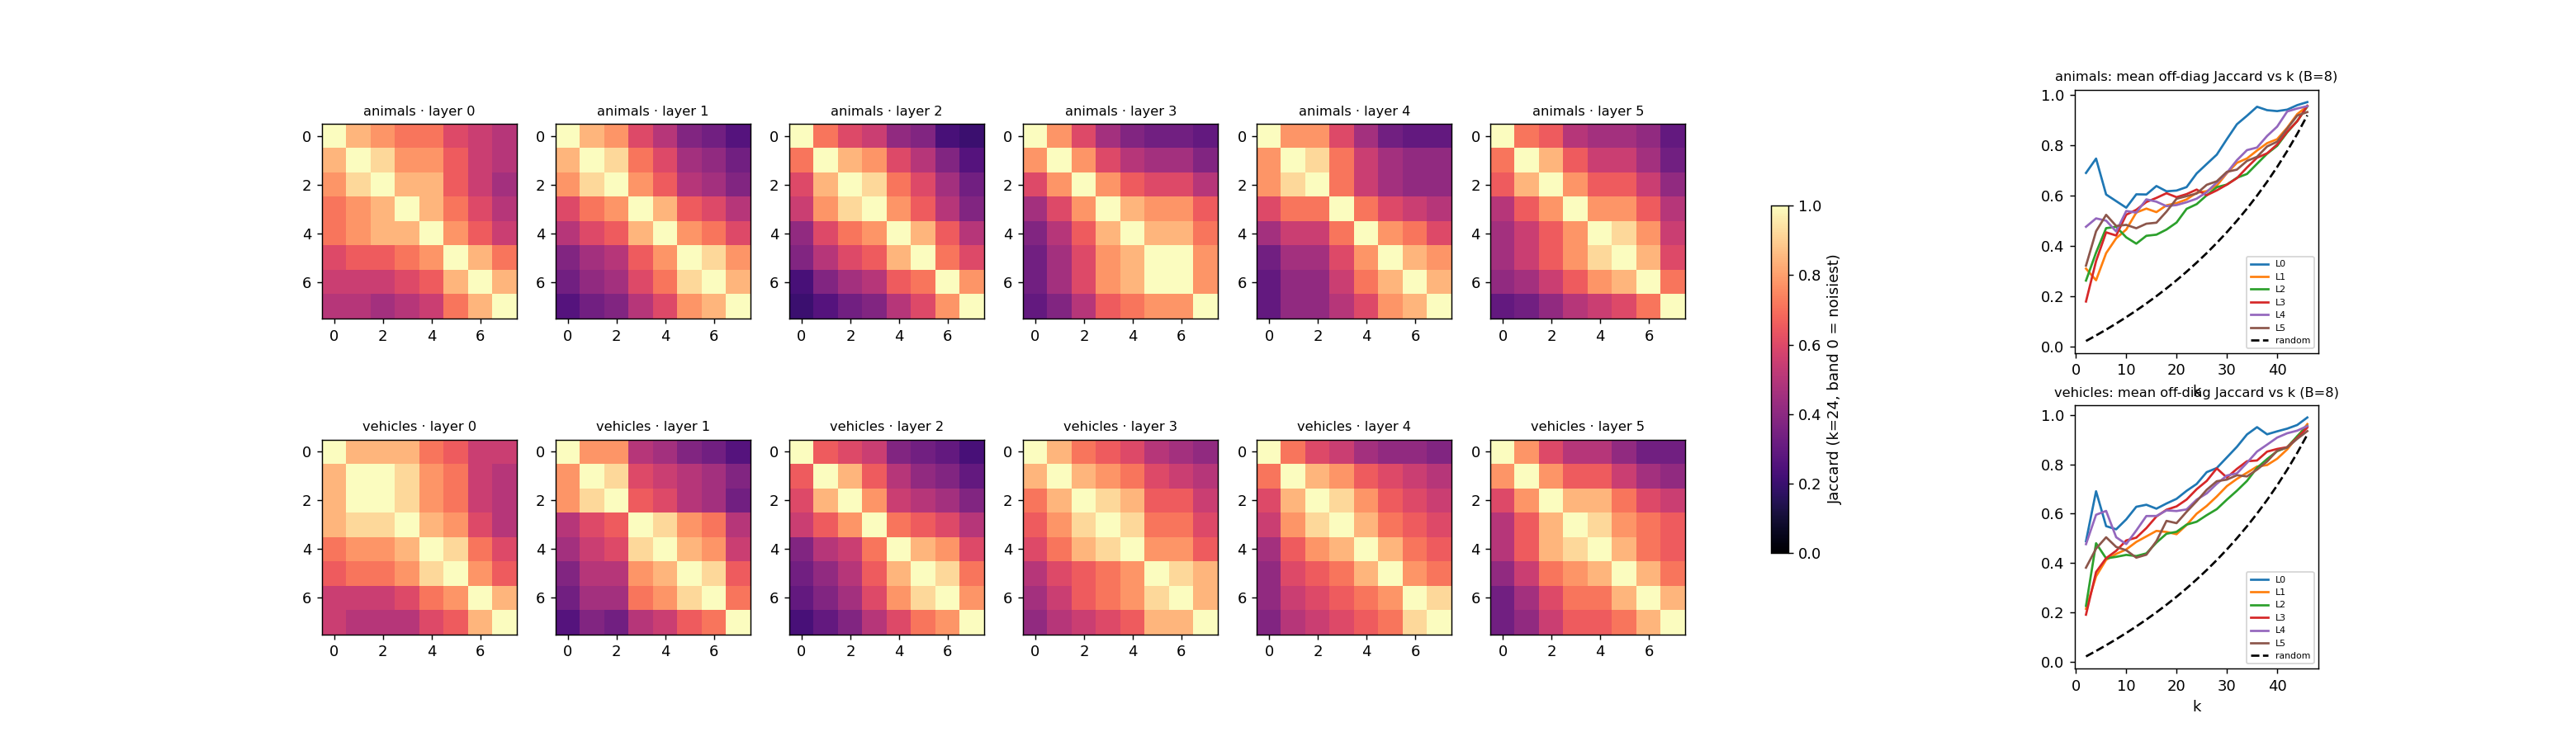
\includegraphics[width=\linewidth]{figures/diagnostic_2.png}
\caption{Band-to-band Jaccard overlap of top-$k$ sets ($B=8$, $k=24$) and mean off-diagonal overlap versus $k$; dashed = random.}\label{fig:jac}
\end{figure}
\begin{figure}[t]\centering
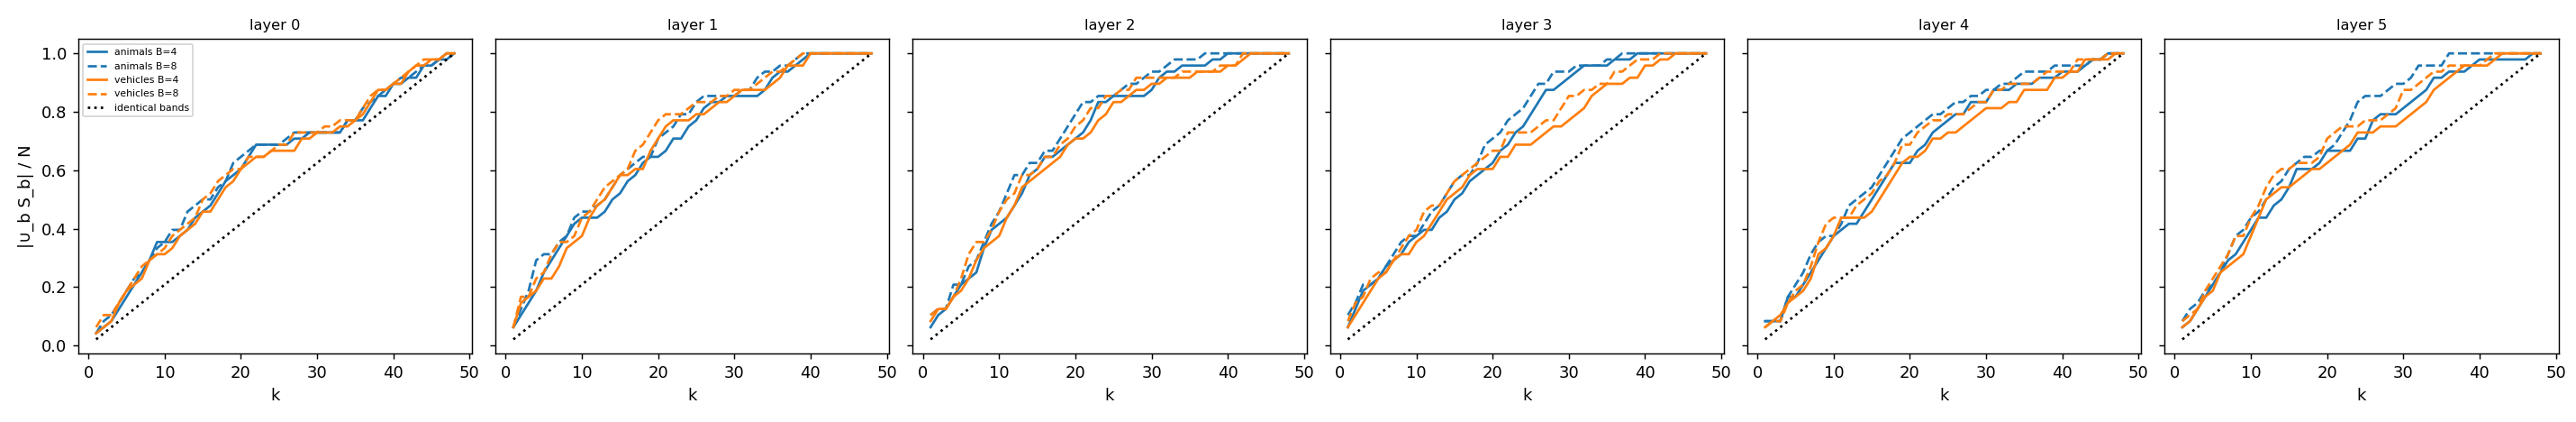
\includegraphics[width=\linewidth]{figures/diagnostic_3.png}
\caption{Union fraction $|\bigcup_b S_b|/N$ versus $k$ for $B=4$ (solid) and $B=8$ (dashed).}\label{fig:union}
\end{figure}

\section{Experiments}\todo{week 6}
\section{Results}\todo{week 7}
\section{Discussion and Limitations}
\todo{week 7. Named limitations so far: 100 vs 69 domain classes (ImageNet-1k is animal-skewed); calibration is conditional-only, no CFG; single backbone.}

\end{document}
